\chapter{Perkembangan Vegetatif Tumbuhan: Meristem dan Pertumbuhan}\label{ch:b2:plant-meristems}

Sebatang pohon ek yang masih kecambah ketika katedralnya dibangun masih
menambahkan selingkar \omterm{def:b2:plant-meristems:wood}{kayu} tiap tahun, masih membuka daun baru tiap
musim semi, masih mendorong ujung akar baru menembus tanahnya. Tidak
ada hewan yang melakukannya; seekor kuda berhenti tumbuh pada umur
empat tahun. Bedanya, sebatang tumbuhan mempertahankan, pada ujung tiap
pucuk dan tiap akarnya serta di dalam sebuah silinder tipis di dalam
tiap batangnya, populasi kecil sel embrionik --- yaitu
\emph{\omterm{def:b2:plant-meristems:meristem}{meristem}} --- yang tidak pernah berhenti membelah, dan yang
membangun tubuh tumbuhannya ke luar dan ke atas selama ia hidup. Bab
ini menelaah bagaimana kedua \omterm{def:b2:plant-meristems:meristem}{meristem} apikalnya ditata dan
dikendalikan, bagaimana sebuah sel tumbuhan tumbuh, bagaimana hormon
memutuskan bentuk sebuah pucuk, dan bagaimana sebuah batang menebal.

\section{Meristem}

\begin{definition}[Meristem dan kedua macam pertumbuhannya]\label{def:b2:plant-meristems:meristem}
\index{meristem}\index{meristem apikal pucuk}%
\index{meristem apikal akar}\index{kambium}
Sebuah \emph{meristem} adalah populasi sel kecil yang tak
terdiferensiasi dan membelah, yang bertahan sepanjang hidup tumbuhannya
dan yang darinya seluruh jaringannya berasal. \emph{Meristem apikal
pucuk} (SAM) pada ujung tiap pucuknya membuat daun, batang, dan, pada
musimnya, \omterm{def:b2:angiosperm-reproduction:flower}{bunga}; \emph{meristem apikal akar} (RAM) di belakang tiap
ujung akarnya membuat akarnya; bersama-sama keduanya menggerakkan
\emph{pertumbuhan primer}, yaitu pemanjangan tumbuhannya. \emph{Meristem
samping} --- \emph{\omterm{def:b2:plant-meristems:wood}{kambium pembuluh}} dan \emph{kambium gabus}, yaitu
silinder tipis di dalam batang dan akarnya --- menggerakkan
\emph{pertumbuhan sekunder}, yaitu penebalan yang membuat \omterm{def:b2:plant-meristems:wood}{kayu} dan
\omterm{def:b2:plant-meristems:wood}{kulit kayu}. Maka pertumbuhan tumbuhannya bersifat \emph{tak tentu}:
meristemnya dapat berlanjut tanpa batas, dan tumbuhannya adalah
organisme bermodul, yang mengulangi satuan daun--buku--ruas--tunas
selama keadaannya mengizinkan. Tiap tunas ketiaknya adalah sebuah SAM
yang dorman, sehingga sebatang tumbuhan mengusung ribuan titik tumbuh
cadangan.
\end{definition}

\begin{proposition}[Pucuk apikalnya]\label{prop:b2:plant-meristems:sam}
\index{filotaksis}\index{primordium daun}\index{plastokron}
SAM adalah sebuah kubah bergaris tengah sepersepuluh milimeter, berisi
beberapa ratus sel. Satu atau dua lapisan luarnya (\emph{tunika}) hanya
membelah pada bidang permukaannya lalu memberi epidermisnya; massa di
bawahnya (\emph{korpus}) membelah pada segala bidang. Pada puncaknya
sebuah \emph{zona pusat} berisi \omterm{def:b2:cell-differentiation:differentiation}{sel punca} yang membelah lambat menyuapi
sebuah \emph{zona tepi} berisi sel yang membelah lebih cepat, dan di
situ \emph{\omterm{prop:b2:plant-meristems:sam}{primordium daun}} muncul sebagai tonjolan pada selang waktu
yang teratur (\emph{plastokron}, berjam-jam sampai berhari-hari) dan
pada sudut yang teratur mengelilingi kubahnya (\emph{filotaksis}:
berhadapan, berkarang, atau berpilin pada sudut emas
\qty{137.5}{\degree}, yang menempatkan tiap daun barunya pada celah
terbesar yang ditinggalkan daun lainnya). Di bawahnya, sebuah
\emph{zona rusuk} membuat empulur lalu memanjangkan batangnya. Sebuah
primordium terbentuk di tempat hormon auksin menimbun di lapisan
permukaannya, dan sembari ia tumbuh ia menguras auksin dari
sekelilingnya, dan itulah sebabnya primordium berikutnya muncul sejauh
mungkin darinya: polanya menata dirinya sendiri.
\end{proposition}

\begin{omfigure}
\begin{tikzpicture}[every node/.style={font=\scriptsize}]
  % dome
  \draw[thick, fill=omExo!12] (-2.2,0) .. controls (-2.2,1.6) and (-0.8,2.6) .. (0,2.6) .. controls (0.8,2.6) and (2.2,1.6) .. (2.2,0) -- (2.2,-1.4) -- (-2.2,-1.4) -- cycle;
  % tunica layers
  \draw[thick, omDef] (-2.2,0) .. controls (-2.2,1.5) and (-0.8,2.45) .. (0,2.45) .. controls (0.8,2.45) and (2.2,1.5) .. (2.2,0);
  \draw[thick, omDef] (-2.05,0) .. controls (-2.05,1.35) and (-0.75,2.3) .. (0,2.3) .. controls (0.75,2.3) and (2.05,1.35) .. (2.05,0);
  % zones
  \draw[thick, dashed, omThm, fill=omThm!15] (0,1.75) ellipse (0.6 and 0.55);
  \draw[thick, dashed, omProp] (0,0.9) ellipse (1.6 and 1.35);
  \draw[thick, dashed, omExo!70!black] (-0.9,-0.9) rectangle (0.9,-0.1);
  % primordia
  \draw[thick, fill=omExo!40] (-2.2,0.4) .. controls (-2.5,1.4) and (-1.6,1.9) .. (-1.55,1.3) .. controls (-1.5,0.9) and (-1.9,0.6) .. (-2.2,0.4);
  \draw[thick, fill=omExo!40] (2.2,0.2) .. controls (2.7,1.0) and (2.1,1.5) .. (1.75,1.1) .. controls (1.6,0.8) and (1.9,0.5) .. (2.2,0.2);
  % labels
  \draw (0.4,2.1) -- (3.2,2.6) node[right, align=left] {zona pusat:\\sel punca yang membelah lambat};
  \draw (1.3,0.5) -- (3.2,1.4) node[right, align=left] {zona tepi:\\pembelahan cepat, primordium daun};
  \draw (0.6,-0.5) -- (3.2,0.0) node[right, align=left] {zona rusuk: empulur,\\pemanjangan batang};
  \draw (-1.7,1.5) -- (-3.0,2.4) node[left, align=right] {primordium\\daun};
  \draw (-1.2,2.05) -- (-3.0,1.2) node[left, align=right] {tunika: pembelahan\\permukaan saja};
  \draw (2.2,0.7) -- (3.2,-1.0) node[right, align=left] {primordium berikutnya,\\\qty{137.5}{\degree} memutar};
\end{tikzpicture}

{\small \omterm{def:b2:plant-meristems:meristem}{Meristem apikal pucuk} dalam potongan: sebuah tunika berlapis
satu atau dua di atas sebuah korpus, sebuah zona pusat berisi \omterm{def:b2:cell-differentiation:differentiation}{sel punca}
pada puncaknya, sebuah zona tepi tempat \omterm{prop:b2:plant-meristems:sam}{primordium daun} menonjol
keluar, dan sebuah zona rusuk di bawahnya.}
\end{omfigure}

\begin{omfigure}
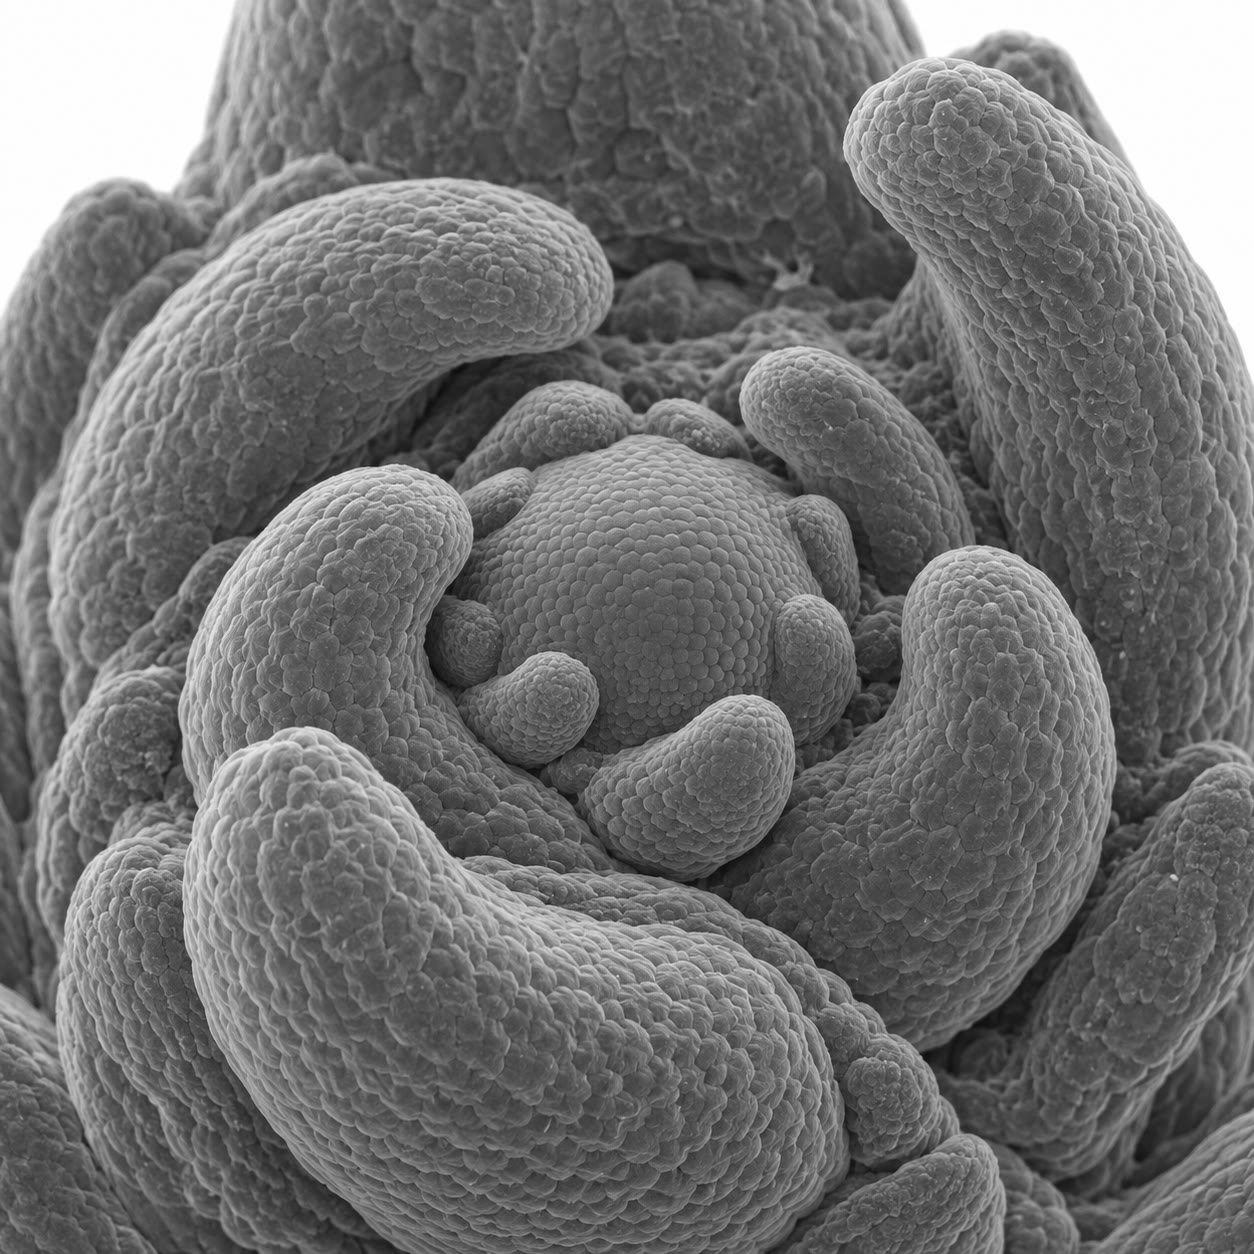
\includegraphics[width=0.44\linewidth]{images/book4/ai/b4-13-shoot-apex-sem.jpg}

{\small Sebuah pucuk apikal di bawah mikroskop elektron payaran: kubah
mulus \omterm{def:b2:plant-meristems:meristem}{meristemnya} dan pilin \omterm{prop:b2:plant-meristems:sam}{primordium daun} di sekelilingnya, tiap yang
baru ditempatkan pada celah yang terlebar.}
\end{omfigure}

\begin{proposition}[Mempertahankan sel puncanya: sebuah gelung umpan balik]\label{prop:b2:plant-meristems:wus}
\index{WUSCHEL}\index{CLAVATA}\index{umpan balik negatif!meristem}
Ukuran lumbung \omterm{def:b2:cell-differentiation:differentiation}{sel puncanya} ditahan tetap oleh sebuah gelung antara dua
gen. Sel tepat di bawah zona pusatnya mengungkapkan \omterm{prop:b2:cell-differentiation:transcriptional}{faktor transkripsi}
\emph{WUSCHEL} (WUS), yang hasilnya bergerak naik ke dalam sel di
atasnya lalu mempertahankannya sebagai \omterm{def:b2:cell-differentiation:differentiation}{sel punca}; \omterm{def:b2:cell-differentiation:differentiation}{sel puncanya} pada
gilirannya menyekresikan sebuah peptida kecil, \emph{CLAVATA3} (CLV3),
yang berdifusi turun, mengikat sebuah reseptor kinase (CLV1) di dalam
sel yang mengungkapkan WUS, lalu menekan WUS. Lebih banyak \omterm{def:b2:cell-differentiation:differentiation}{sel punca}
berarti lebih banyak CLV3, lebih sedikit WUS, lebih sedikit \omterm{def:b2:cell-differentiation:differentiation}{sel punca};
lebih sedikit \omterm{def:b2:cell-differentiation:differentiation}{sel punca} berarti lebih sedikit CLV3, lebih banyak WUS,
lebih banyak \omterm{def:b2:cell-differentiation:differentiation}{sel punca}. Maka lumbungnya adalah sebuah besaran yang
teratur, seperti gonadotropin \cref{ch:b2:reproductive-hormones}, dan
tata nalar yang sama --- sebuah isyarat dari populasi yang diatur yang
menekan faktor yang membuatnya --- juga menahan \omterm{def:b2:plant-meristems:meristem}{meristem} akarnya.
\end{proposition}
\begin{proof}[Bukti eksperimental]
Mutan \emph{clavata} Arabidopsis (Clark, Meyerowitz, 1990-an) memiliki
\omterm{def:b2:plant-meristems:meristem}{meristem} yang membengkak berlipat-lipat ukuran normalnya, dengan daun
tambahan, organ \omterm{def:b2:angiosperm-reproduction:flower}{bunga} tambahan, dan batang yang berfasiasi (pipih
seperti pita): remnya lenyap. Mutan \emph{wuschel} membuat sebuah
\omterm{def:b2:plant-meristems:meristem}{meristem} yang berhenti sesudah beberapa daun lalu membentuk \omterm{def:b2:plant-meristems:meristem}{meristem}
baru, yang masing-masing berhenti pada gilirannya: pedal gasnya lenyap.
Pada mutan gandanya, \omterm{def:b2:meiosis-heredity:vocabulary}{fenotipe} \emph{wuschel} yang menang, sehingga WUS
berada di hilir CLV; dan peptida CLV3 yang diberikan pada sebuah pucuk
tipe liar menekan WUS dalam hitungan jam.
\end{proof}

\begin{proposition}[Pucuk akarnya]\label{prop:b2:plant-meristems:ram}
\index{tudung akar}\index{pusat diam}\index{zona pemanjangan}\index{rambut akar}
Sebuah akar tumbuh dari sebuah \omterm{def:b2:plant-meristems:meristem}{meristem} yang terlindung di balik
sebuah \emph{\omterm{prop:b2:plant-meristems:ram}{tudung akar}}, yang selnya terkelupas sembari ujungnya
mendorong menembus tanahnya dan yang menyekresikan lendir pelumas serta
mengindera gravitasi (butiran pati yang mengendap di dalam selnya). Di
pusat \omterm{def:b2:plant-meristems:meristem}{meristemnya}, sebuah \emph{\omterm{prop:b2:plant-meristems:ram}{pusat diam}} berisi beberapa ratus sel
hanya membelah sesekali; ia mempertahankan sel pemula di sekelilingnya
--- sel pemula tudungnya, epidermisnya, korteksnya, dan silinder
pembuluhnya --- sebagai \omterm{def:b2:cell-differentiation:differentiation}{sel punca}, sama seperti WUS mempertahankan \omterm{def:b2:cell-differentiation:differentiation}{sel
punca} pucuknya. Di belakang \omterm{def:b2:plant-meristems:meristem}{meristemnya} datang \emph{\omterm{prop:b2:plant-meristems:ram}{zona
pemanjangan}}, yaitu beberapa milimeter tempat selnya memanjang sepuluh
sampai dua puluh kali lipat, yang mendorong ujungnya maju; lalu
\emph{zona \omterm{def:b2:cell-differentiation:differentiation}{diferensiasi}}, tempat epidermisnya menumbuhkan \emph{\omterm{prop:b2:plant-meristems:ram}{rambut
akar}} dan xilem serta floemnya matang. Akar samping muncul bukan pada
ujungnya melainkan dari perisikel, jauh di dalam akar yang matang,
berseberangan dengan kutub xilemnya, lalu mendorong keluar menembus
korteksnya. Auksin, yang dibuat di pucuknya lalu dibawa turun,
menimbun pada ujungnya lalu menata seluruh susunannya; \omterm{prop:b2:plant-meristems:ram}{pusat diamnya}
duduk pada maksimumnya.
\end{proposition}

\begin{omfigure}
\begin{tikzpicture}[every node/.style={font=\scriptsize}]
  % root outline
  \draw[thick, fill=omExo!10] (-1.0,4.5) -- (-1.0,0.6) .. controls (-1.0,-0.4) and (1.0,-0.4) .. (1.0,0.6) -- (1.0,4.5);
  % root cap
  \draw[thick, fill=omExo!45] (-0.9,0.8) .. controls (-1.1,-0.1) and (1.1,-0.1) .. (0.9,0.8) .. controls (0.5,0.4) and (-0.5,0.4) .. (-0.9,0.8);
  % meristem
  \fill[omThm!25] (-0.85,0.8) rectangle (0.85,1.7);
  \fill[omThm!70] (0,0.95) ellipse (0.25 and 0.12);
  % elongation zone
  \fill[omProp!20] (-0.85,1.7) rectangle (0.85,3.0);
  % differentiation zone with root hairs and vascular strand
  \fill[omDef!15] (-0.85,3.0) rectangle (0.85,4.5);
  \fill[omDef!50] (-0.15,3.0) rectangle (0.15,4.5);
  \foreach \y in {3.2,3.5,3.8,4.1,4.4} { \draw[omDef!80!black] (1.0,\y) -- (1.7,\y+0.1); \draw[omDef!80!black] (-1.0,\y) -- (-1.7,\y+0.1); }
  % lateral root primordium
  \draw[thick, fill=omThm!30] (0.15,4.0) .. controls (0.5,3.9) and (0.8,4.1) .. (0.9,4.3) .. controls (0.7,4.35) and (0.4,4.3) .. (0.15,4.3);
  % labels
  \draw (0.5,0.4) -- (2.2,0.2) node[right] {tudung akar};
  \draw (0.25,0.95) -- (2.2,0.9) node[right] {pusat diam};
  \draw (0.85,1.4) -- (2.2,1.5) node[right] {meristem (pembelahan)};
  \draw (0.85,2.4) -- (2.2,2.3) node[right, align=left] {zona pemanjangan:\\sel memanjang $10\times$};
  \draw (1.5,3.6) -- (2.2,3.4) node[right] {rambut akar};
  \draw (0.0,4.2) -- (2.2,4.2) node[right] {silinder pembuluh};
  \draw (0.7,4.3) -- (2.2,4.9) node[right, align=left] {primordium akar samping\\(dari perisikelnya)};
  \draw[->, thick] (-2.4,4.5) -- (-2.4,0.6); \node[left, rotate=90, anchor=south] at (-2.5,2.5) {auksin mengalir ke ujungnya};
\end{tikzpicture}

{\small Ujung akarnya: tudung, \omterm{def:b2:plant-meristems:meristem}{meristem} beserta \omterm{prop:b2:plant-meristems:ram}{pusat diamnya},
\omterm{prop:b2:plant-meristems:ram}{zona pemanjangan}, dan zona \omterm{def:b2:cell-differentiation:differentiation}{diferensiasi} dengan \omterm{prop:b2:plant-meristems:ram}{rambut akar} serta
pembuluh yang matang. Akar samping mulai jauh di dalamnya, dari perisikelnya.}
\end{omfigure}

\begin{omfigure}
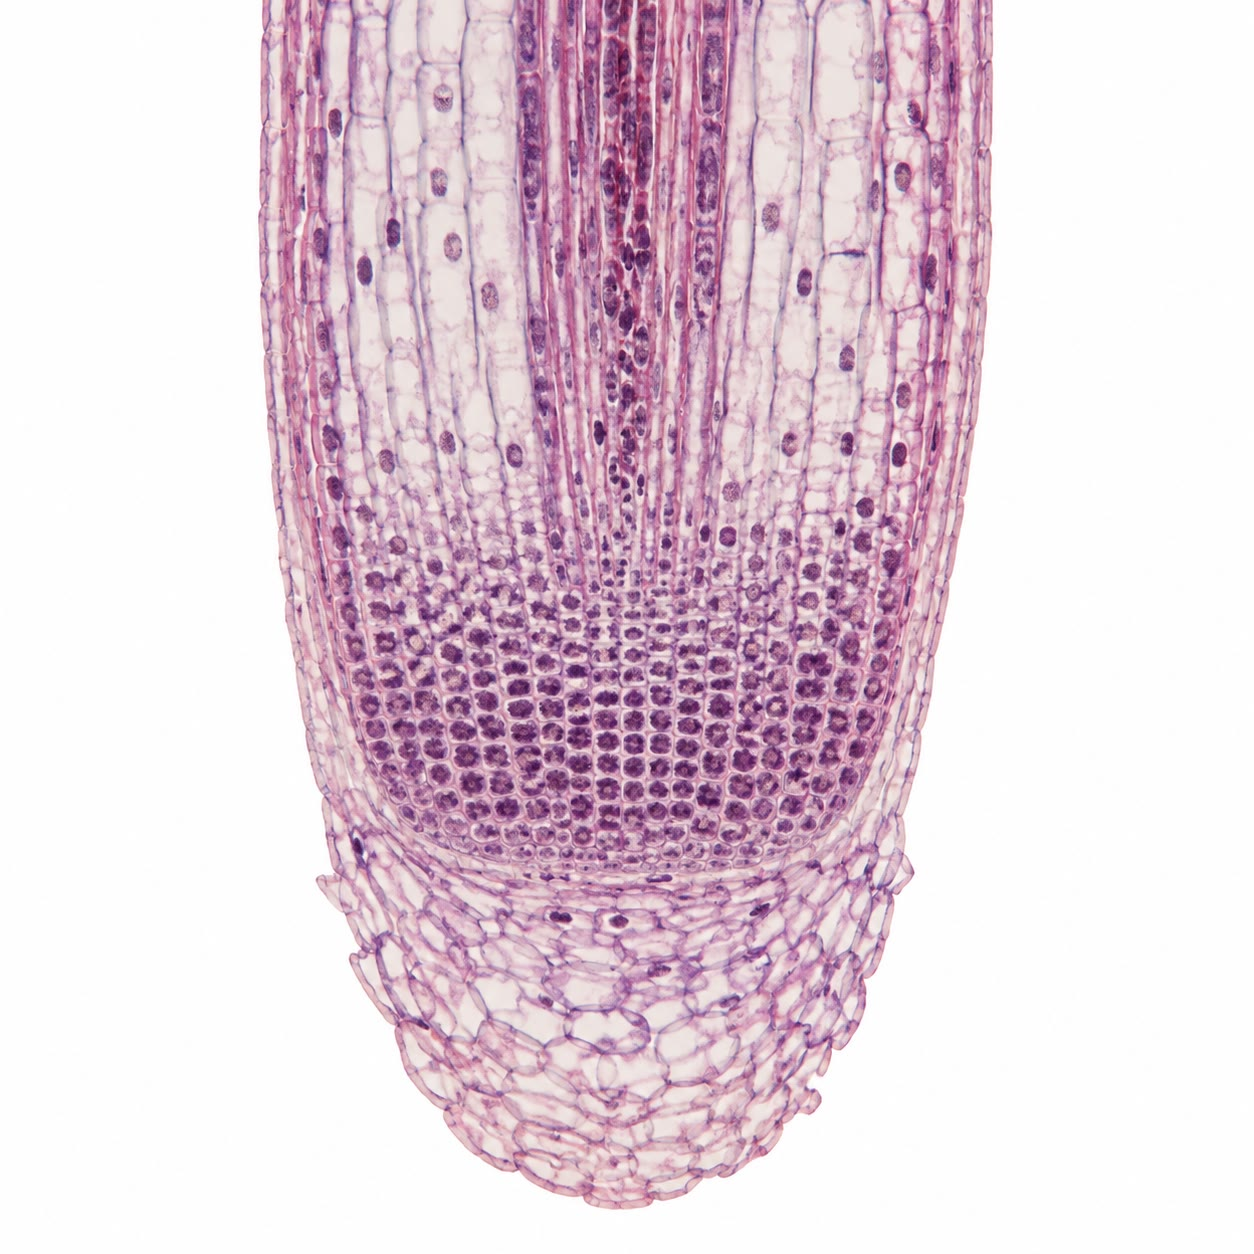
\includegraphics[width=0.42\linewidth]{images/book4/ai/b4-13-root-tip.jpg}

{\small Sebuah ujung akar dalam potongan membujur: sel tudungnya yang
longgar, \omterm{def:b2:plant-meristems:meristem}{meristemnya} yang rapat dengan inti gelapnya, dan sel yang
memanjang di atasnya.}
\end{omfigure}

\section{Bagaimana sebuah sel tumbuhan tumbuh}

\begin{theorem}[Persamaan Lockhart]\label{thm:b2:plant-meristems:lockhart}
\index{turgor}\index{dinding sel!keterentangan}\index{persamaan Lockhart}
Sebuah sel tumbuhan tumbuh dengan meregangkan dindingnya di bawah
tekanan isinya sendiri. Dindingnya hanya mengalah secara tak terbalikkan
di atas sebuah turgor ambang $Y$, dan lalu pada laju yang sebanding
dengan kelebihannya: laju pertumbuhan nisbi sebuah sel sepanjang $L$
adalah
\[
\frac{1}{L}\frac{\mathrm{d}L}{\mathrm{d}t} = \phi\,(P - Y) \quad (P > Y),
\]
dengan $P$ sebagai tekanan turgornya dan $\phi$ sebagai
\emph{keterentangan} dindingnya. Maka pertumbuhannya dikendalikan dari
dua sisi: oleh air, yang menetapkan $P$ (sel yang layu berhenti
tumbuh), dan oleh dindingnya, yang menetapkan $\phi$ dan $Y$ --- dan
dindingnyalah yang menjadi tempat hormon bekerja. Auksin membuat selnya
memompa proton ke dalam dindingnya; asamnya mengaktifkan
\emph{ekspansin}, yaitu protein yang melonggarkan ikatan antara fibril
selulosanya dan matriksnya, sehingga menaikkan $\phi$ dan menurunkan
$Y$ dalam hitungan menit (\emph{pertumbuhan asam}). Dengan $\phi =
\qty{0.1}{h^{-1}.MPa^{-1}}$, $Y = \qty{0.3}{MPa}$ dan $P =
\qty{0.6}{MPa}$, sebuah sel memanjang \qty{3}{\%} tiap jam lalu berlipat
dua dalam sehari; di dalam \omterm{prop:b2:plant-meristems:ram}{zona pemanjangan} sebuah akar, tempat lajunya
beberapa kali lebih tinggi, sebuah sel memanjang sepuluh kali lipat
dalam beberapa jam.
\end{theorem}
\begin{proof}
Dindingnya adalah bahan viskoplastik: di bawah tegangan luluhnya ia
berubah bentuk secara elastik lalu pulih, di atasnya ia mengalir pada
laju yang sebanding dengan kelebihan tegangannya. Tegangan di dalam
dindingnya sebanding dengan tekanan turgornya (bagi sebuah silinder
berjari-jari $r$ dan berdinding setebal $w$, tegangan gelangnya adalah
$Pr/w$), sehingga laju regangan plastiknya sebanding dengan $P - Y$
dengan sebuah tetapan $\phi$ yang menyerap geometrinya dan sifat bahan
dindingnya. Laju regangannya menurut definisi adalah
$(1/L)\,\mathrm{d}L/\mathrm{d}t$. Secara angka,
$0.1\times(0.6 - 0.3) = \qty{0.03}{h^{-1}}$, dan $L$ berlipat dua
ketika $0.03\,t = \ln 2$, yaitu $t = \qty{23}{h}$.
\end{proof}

\begin{omfigure}
\begin{tikzpicture}
\begin{axis}[
  width=0.7\linewidth, height=5.4cm,
  axis x line=bottom, axis y line=left,
  xmin=0, xmax=1.0, ymin=0, ymax=0.09,
  xlabel={tekanan turgor $P$ (\unit{MPa})}, ylabel={laju pertumbuhan nisbi (\unit{h^{-1}})},
  xlabel style={font=\small, at={(axis description cs:0.5,-0.13)}, anchor=north},
  ylabel style={font=\small},
  tick label style={font=\small}, xtick={0,0.3,0.6,0.9}, ytick={0,0.03,0.06,0.09},
  yticklabels={0,0.03,0.06,0.09}, scaled y ticks=false,
  legend style={font=\scriptsize, at={(0.03,0.97)}, anchor=north west, draw=none},
  clip=false,
]
\addplot[very thick, omDef, domain=0:0.3, samples=2, forget plot] {0};
\addplot[very thick, omDef, domain=0.3:1.0, samples=2] {0.1*(x-0.3)};
\addlegendentry{$\phi = 0.1$, $Y = 0.3$}
\addplot[very thick, omThm, domain=0:0.2, samples=2, forget plot] {0};
\addplot[very thick, omThm, domain=0.2:0.65, samples=2] {0.2*(x-0.2)};
\addlegendentry{dengan auksin: $\phi = 0.2$, $Y = 0.2$}
\draw[dashed, gray] (axis cs:0.6,0) -- (axis cs:0.6,0.03); \node[font=\scriptsize, anchor=west] at (axis cs:0.61,0.015) {$P$ yang khas};
\end{axis}
\end{tikzpicture}

{\small Hukum Lockhart: tanpa pertumbuhan di bawah turgor luluhnya,
lalu sebuah laju yang sebanding dengan kelebihannya. Auksin, dengan
melonggarkan dindingnya, menurunkan ambangnya dan mencuramkan garisnya,
dan pada turgor yang sama selnya tumbuh beberapa kali lebih cepat.}
\end{omfigure}

\begin{example}[Dari mana airnya datang]\label{ex:b2:plant-meristems:water}
Sembari dindingnya mengalah, turgornya akan turun dan pertumbuhannya
berhenti, seandainya air tidak masuk mengimbanginya: sel yang tumbuh
adalah sebuah kebocoran yang mengisi dirinya sendiri. Airnya datang
dari xilemnya, menuruni sebuah landaian potensial air yang kecil, dan
laju masuknya ditetapkan keterhantaran hidraulik membrannya;
pertumbuhannya tercepat pada malam hari, ketika transpirasinya rendah
dan turgornya tinggi, dan sehelai daun jagung dapat memanjang
\qty{10}{cm} antara senja dan fajar. Di bawah kekeringan, selnya
membuat zat terlarut (\emph{penyesuaian osmosis}) untuk menjaga $P$
tetap di atas $Y$, dan ketika hal itu gagal, daunnya berhenti tumbuh
beberapa hari sebelum ia layu.
\end{example}

\section{Hormon dan bentuk pucuknya}

\begin{proposition}[Auksin dan dominansi apikal]\label{prop:b2:plant-meristems:apical}
\index{auksin}\index{dominansi apikal}%
\index{pengangkutan auksin terkutub}\index{sitokinin}
\emph{Auksin} (asam indol-3-asetat) dibuat di pucuk apikalnya dan di
daun mudanya lalu dibawa turun menyusuri batangnya, sel demi sel, pada
kira-kira \qty{1}{cm/h}, oleh protein pengangkut (PIN) yang terpasang
pada ujung bawah tiap selnya --- sebuah \emph{pengangkutan terkutub}
yang memberi tumbuhannya sebuah sumbu atas ke bawah. Aliran auksin yang
menurun dari pucuknya menjaga tunas ketiak di bawahnya tetap dorman
(\emph{\omterm{prop:b2:plant-meristems:apical}{dominansi apikal}}), sebagian dengan mencegahnya mengekspor
auksinnya sendiri ke dalam batangnya, sebagian dengan mengimbas
strigolakton dan menekan sitokinin. Potonglah pucuknya dan tunas yang
terdekat dengan potongannya tumbuh keluar dalam beberapa hari, sehingga
tumbuhannya menjadi rimbun --- dan itulah yang dimanfaatkan pemangkasan
dan pencomotan. \emph{Sitokinin}, yang dibuat di ujung akarnya lalu
dibawa naik di dalam xilemnya, memacu pertumbuhan tunas dan pembelahan
sel; \emph{giberelin} memanjangkan ruas batangnya (kacang ercis kerdil
dan gandum setengah kerdil Revolusi Hijau cacat dalam membuat atau
mengindera giberelin); asam absisat dan etilena mengerem pertumbuhannya
di bawah tekanan. Bentuk pucuknya --- tinggi atau rimbun, tegak atau
melebar --- adalah hasil perundingan di antara isyarat ini, dan
keseimbangan akar terhadap pucuknya ditetapkan auksin yang turun
melawan sitokinin yang naik.
\end{proposition}
\begin{proof}[Bukti eksperimental]
Thimann dan Skoog (1934) memotong pucuk apikal tumbuhan buncis: tunas
sampingnya tumbuh. Sebongkah agar berisi auksin, yang ditaruh pada
tunggul potongannya, menjaganya tetap dorman seperti yang dilakukan
pucuknya; agar polos tidak. Went (1928) telah lebih dahulu mengukur
auksin lewat bengkokan yang dihasilkannya pada koleoptil gandum yang
dipenggal ketika ditaruh pada satu sisi tunggulnya --- bioasai pertama
sebuah hormon tumbuhan, dan asal namanya, dari bahasa Yunani yang
berarti ``tumbuh''. Kekutuban pengangkutannya ditunjukkan dengan
menaruh agar berauksin pada satu ujung sepotong batang lalu
menemukannya di dalam bongkah penerima pada ujung yang lain hanya
ketika potongannya berarah pucuk ke atas, bagaimanapun potongannya
diputar di dalam medan gravitasinya.
\end{proof}

\begin{omfigure}
\begin{tikzpicture}[every node/.style={font=\scriptsize}, >=stealth]
  \foreach \x/\lab/\apex/\aux in {0/{utuh: pucuk apikal ada,\\tunas dorman}/1/0, 4.2/{dipenggal:\\tunas tumbuh keluar}/0/0, 8.4/{dipenggal + auksin\\pada tunggulnya: dorman}/0/1} {
    \begin{scope}[xshift=\x cm]
      \draw[very thick, omExo!70!black] (0,0) -- (0,3.4);
      \foreach \y in {0.8,1.6,2.4} { \draw[thick, omExo!70!black] (0,\y) -- (-0.8,\y+0.4); \draw[thick, omExo!70!black] (0,\y+0.4) -- (0.8,\y+0.8); }
      \ifnum\apex=1 \draw[thick, fill=omThm!40] (0,3.5) ellipse (0.25 and 0.3); \draw[->, thick, omThm] (0.35,3.2) -- (0.35,1.0); \node[omThm, right] at (0.4,2.1) {auksin}; \fi
      \ifnum\apex=0 \draw[thick] (-0.3,3.4) -- (0.3,3.4); \fi
      \ifnum\aux=1 \draw[thick, fill=omThm!40] (-0.25,3.4) rectangle (0.25,3.75); \node[omThm, right] at (0.3,3.6) {agar auksin}; \draw[->, thick, omThm] (0.35,3.2) -- (0.35,1.0); \fi
      \ifnum\apex=1 \foreach \y in {0.8,1.6,2.4} \fill[gray!60] (-0.12,\y+0.1) circle (0.08); \fi
      \ifnum\aux=1 \foreach \y in {0.8,1.6,2.4} \fill[gray!60] (-0.12,\y+0.1) circle (0.08); \fi
      \ifnum\apex=0 \ifnum\aux=0 \foreach \y in {0.8,1.6,2.4} { \draw[thick, omExo!70!black] (-0.1,\y+0.1) -- (-0.7,\y+0.9); \draw[thick, omExo!70!black] (-0.7,\y+0.9) -- (-1.0,\y+1.1); \draw[thick, omExo!70!black] (-0.7,\y+0.9) -- (-0.75,\y+1.25); } \fi\fi
      \node[below, align=center] at (0,-0.3) {\lab};
    \end{scope}
  }
\end{tikzpicture}

{\small \omterm{prop:b2:plant-meristems:apical}{Dominansi apikal}, percobaan Thimann--Skoog. Pucuk apikalnya
menjaga tunas ketiaknya tetap dorman; membuangnya melepaskannya;
auksin pada tunggul potongannya menggantikan pucuk apikalnya.}
\end{omfigure}

\begin{example}[Isyarat cepat, molekul lambat]\label{ex:b2:plant-meristems:transport}
Pengangkutan terkutub memindahkan auksin \qty{1}{cm} dalam sejam;
difusi semata akan memakan, bagi sentimeter yang sama, $t = x^2/2D = 10^{-4}/(2\times
10^{-9}) = \qty{5e4}{s}$ --- empat belas jam --- dan
bagi sepuluh sentimeter menuju sebuah tunas yang lebih rendah, enam
puluh hari. Pompa dan penyambung pengangkut PIN itulah yang membuat
sebuah isyarat hormon dapat dipakai sepanjang tumbuhannya; pengangkut
yang sama, yang dipindahkan ke sisi batang yang ternaungi,
membengkokkannya ke arah cahayanya (\cref{ch:b2:plant-plasticity}).
\end{example}

\section{Pertumbuhan sekunder: kayu dan kulit kayu}

\begin{definition}[Kambium pembuluh dan kayu]\label{def:b2:plant-meristems:wood}
\index{kambium pembuluh}\index{kayu}\index{lingkaran tahun}%
\index{kulit kayu}\index{periderm}
Pada sebuah batang berkayu, untaian xilem dan floem primernya
disatukan, pada tahun pertamanya, menjadi sebuah silinder sinambung
berisi sel yang membelah, yaitu \emph{\omterm{def:b2:plant-meristems:meristem}{kambium} pembuluh}. Selnya
membelah secara tangensial, menambahkan \emph{xilem sekunder} ---
yaitu \emph{kayu} --- ke sebelah dalamnya dan \emph{floem sekunder} ke
sebelah luarnya, sehingga \omterm{def:b2:plant-meristems:meristem}{kambiumnya} bergerak ke luar sembari batangnya
menebal, serta menambahkan pembelahan jejari sesekali untuk memperlebar
lingkarannya. Di iklim bermusim, kayu yang diletakkan pada musim semi
memiliki pembuluh yang lebar dan berdinding tipis (\emph{kayu awal})
dan kayu musim panas memiliki pembuluh yang sempit dan berdinding tebal
(\emph{kayu akhir}), sehingga tiap tahunnya meninggalkan sebuah
\emph{lingkaran tahun} yang terlihat; lingkarannya merekam umur
pohonnya dan, dalam lebarnya, iklim tiap tahunnya (dendrokronologi).
Hanya lingkaran luarnya, yaitu \emph{kayu gubal}, yang menghantarkan;
lingkaran dalamnya, yaitu \emph{kayu teras}, sudah mati, tersumbat dan
menggelap oleh resin dan tanin, serta berperan sebagai rangka pohonnya.
Di luar floemnya, sebuah \omterm{def:b2:plant-meristems:meristem}{meristem} samping kedua, yaitu \emph{\omterm{def:b2:plant-meristems:meristem}{kambium}
gabus}, membuat \emph{periderm} --- yaitu lapisan sel gabus, mati dan
kedap air oleh suberin --- yang bersama floem lamanya menjadi
\emph{kulit kayu}. Maka sebuah batang adalah selaput hidup tipis berisi
\omterm{def:b2:plant-meristems:meristem}{kambium}, kayu gubal, dan floem di sekeliling sebuah teras yang mati, di
bawah sebuah kulit yang mati.
\end{definition}

\begin{omfigure}
\begin{tikzpicture}[every node/.style={font=\scriptsize}]
  \fill[omExo!60] (0,0) circle (3.0);
  \fill[omDef!20] (0,0) circle (2.75);
  \fill[omDef!35] (0,0) circle (2.2);
  \foreach \r in {0.4,0.7,1.0,1.3,1.6,1.9,2.2} \draw[omDef!80!black, thin] (0,0) circle (\r);
  \fill[omExo!80!black] (0,0) circle (1.3);
  \foreach \r in {0.4,0.7,1.0} \draw[omExo!40, thin] (0,0) circle (\r);
  \draw[very thick, omThm] (0,0) circle (2.5);
  \draw (2.9,0.6) -- (3.9,1.6) node[right, align=left] {kulit kayu: gabus (periderm)\\dan floem lama};
  \draw (2.62,0.0) -- (3.9,0.6) node[right] {floem sekunder, hidup};
  \draw (2.5,-0.4) -- (3.9,-0.4) node[right] {kambium pembuluh (merah)};
  \draw (1.9,-1.1) -- (3.9,-1.4) node[right, align=left] {kayu gubal: lingkaran baru,\\menghantarkan};
  \draw (0.5,-0.9) -- (3.9,-2.4) node[right, align=left] {kayu teras: lingkaran lama,\\mati, tersumbat};
  \draw (-1.7,1.5) -- (-3.6,2.4) node[left, align=right] {satu lingkaran tahun:\\kayu awal yang pucat,\\kayu akhir yang gelap};
\end{tikzpicture}

{\small Sebuah batang dalam potongan melintang. \omterm{def:b2:plant-meristems:meristem}{Kambiumnya} (merah)
menambahkan \omterm{def:b2:plant-meristems:wood}{kayu} ke dalam dan floem ke luar tiap tahunnya; lingkaran
barunya menghantarkan, lingkaran lamanya membentuk \omterm{def:b2:plant-meristems:wood}{kayu} teras yang
mati; gabus dan floem lamanya membuat \omterm{def:b2:plant-meristems:wood}{kulit kayunya}.}
\end{omfigure}

\begin{theorem}[Mengapa pohon tua menambahkan lebih banyak kayu]\label{thm:b2:plant-meristems:rings}
Sebuah batang berjari-jari $r$ dan bertinggi $h$ yang \omterm{def:b2:plant-meristems:meristem}{kambiumnya}
menambahkan selingkar setebal $\Delta r$ tiap tahun memperoleh volume
\omterm{def:b2:plant-meristems:wood}{kayu}
\[
\Delta V \approx 2\pi r\,h\,\Delta r
\]
tiap tahun: bagi lebar lingkaran yang tetap, tambahan tahunannya tumbuh
sebanding dengan jari-jarinya, dan sebatang pohon berjari-jari
\qty{50}{cm} menambahkan \omterm{def:b2:plant-meristems:wood}{kayu} sepuluh kali lipat \omterm{def:b2:plant-meristems:wood}{kayu} pohon
berjari-jari \qty{5}{cm}, meskipun lingkarannya tidak lebih lebar.
Sebuah batang berjari-jari \qty{25}{cm} dan bertinggi \qty{10}{m} yang
menambahkan \qty{4}{mm} tiap tahun memperoleh \qty{0.063}{m^3}, yaitu
kira-kira \qty{30}{kg} \omterm{def:b2:plant-meristems:wood}{kayu} kering --- \qty{15}{kg} karbon, yang
ditarik dari udara oleh tajuknya dalam satu musim.
\end{theorem}
\begin{proof}
\omterm{def:b2:plant-meristems:wood}{Kayu} yang ditambahkannya adalah sebuah selaput silinder berkeliling
$2\pi r$, bertebal $\Delta r$, dan bertinggi $h$; volumenya adalah
$2\pi r h\Delta r$ sampai orde pertama dalam $\Delta r$ (tepatnya
$\pi h[(r + \Delta r)^2 - r^2]
= \pi h(2r\Delta r + \Delta r^2)$). Dengan $r = 0.25$, $h = 10$,
$\Delta r = 0.004$: $2\pi\times 0.25\times 10\times 0.004 =
\qty{0.063}{m^3}$; pada \qty{500}{kg/m^3} kering, \qty{31}{kg},
separuhnya karbon.
\end{proof}

\begin{omfigure}
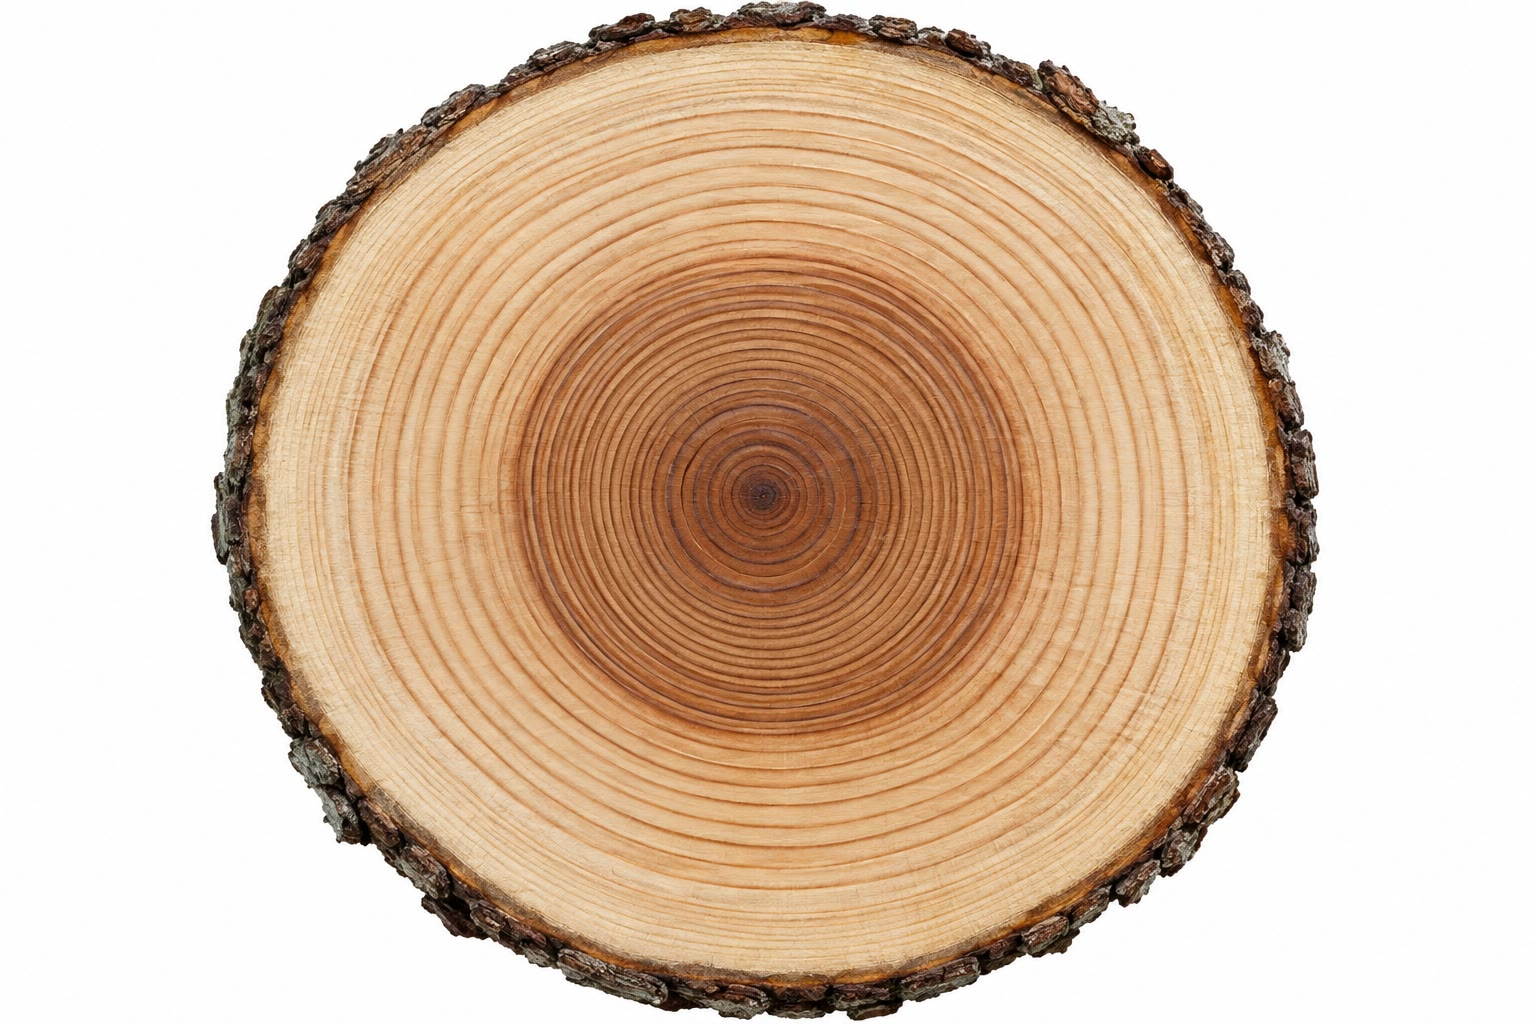
\includegraphics[width=0.5\linewidth]{images/book4/ai/b4-13-wood-rings.jpg}

{\small Sebuah batang pinus dalam potongan melintang: \omterm{def:b2:plant-meristems:wood}{lingkaran
tahunnya}, tiap lingkarannya sebuah pita pucat \omterm{def:b2:plant-meristems:wood}{kayu} awal dan sebuah pita
gelap \omterm{def:b2:plant-meristems:wood}{kayu} akhir, \omterm{def:b2:plant-meristems:wood}{kayu} terasnya yang lebih gelap, dan \omterm{def:b2:plant-meristems:wood}{kulit kayunya}.}
\end{omfigure}

\section{Latihan}

\begin{exercise}[$\star$]\label{exo:b2:plant-meristems:1}
Definisikan \omterm{def:b2:plant-meristems:meristem}{meristem}, lalu sebutkan keempat \omterm{def:b2:plant-meristems:meristem}{meristem} sebatang tumbuhan
berkayu beserta apa yang dihasilkan masing-masingnya.
\end{exercise}

\begin{exercise}[$\star$]\label{exo:b2:plant-meristems:2}
Daftarkan zona sebuah ujung akar dari tudungnya ke atas, beserta apa
yang terjadi pada sebuah sel di tiap zonanya. Dari mana akar sampingnya
datang?
\end{exercise}

\begin{exercise}[$\star$]\label{exo:b2:plant-meristems:3}
Perikanlah percobaan Thimann--Skoog, kendalinya, dan kesimpulannya.
\end{exercise}

\begin{exercise}[$\star$]\label{exo:b2:plant-meristems:4}
Sebuah potongan batang memperlihatkan 60 lingkaran, 15 lingkaran
terluarnya pucat dan sisanya gelap. Berikan umur pohonnya, umur \omterm{def:b2:plant-meristems:wood}{kayu}
gubalnya, lalu katakan bagian mana batangnya yang hidup.
\end{exercise}

\begin{exercise}[$\star\star$]\label{exo:b2:plant-meristems:5}
Dengan $\phi = \qty{0.1}{h^{-1}.MPa^{-1}}$, $Y = \qty{0.3}{MPa}$,
hitunglah laju pertumbuhan nisbinya pada $P = 0.4$, $0.6$, dan
\qty{0.8}{MPa}, serta waktu pelipatduaannya pada masing-masingnya.
Sebuah kekeringan menurunkan $P$ ke \qty{0.25}{MPa}: apa yang terjadi?
\end{exercise}

\begin{exercise}[$\star\star$]\label{exo:b2:plant-meristems:6}
Daun yang berturut-turut muncul pada \qty{137.5}{\degree} satu dari
yang lain. Hitunglah kedudukan sudut daun 1 sampai 8 (modulo
\qty{360}{\degree}) lalu tunjukkan bahwa tidak ada dua daun dari
kedelapan daun pertamanya yang terletak dalam selang
\qty{20}{\degree} satu sama lain. Mengapa hal ini berarti bagi
tumbuhannya?
\end{exercise}

\begin{exercise}[$\star\star$]\label{exo:b2:plant-meristems:7}
Sebatang pohon setinggi \qty{12}{m} menambahkan lingkaran setebal
\qty{3}{mm}. Hitunglah \omterm{def:b2:plant-meristems:wood}{kayu} yang ditambahkan pada tahun jari-jarinya
\qty{5}{cm} dan pada tahun jari-jarinya \qty{40}{cm}, serta karbon yang
bersesuaian (massa jenis keringnya \qty{500}{kg/m^3}, separuhnya karbon).
\end{exercise}

\begin{exercise}[$\star\star$]\label{exo:b2:plant-meristems:8}
Ramalkanlah \omterm{def:b2:meiosis-heredity:vocabulary}{fenotipe} sebuah mutan \emph{clv3}, sebuah mutan \emph{wus},
dan mutan gandanya, lalu jelaskan urutan kedua gennya di dalam
gelungnya dari mutan gandanya.
\end{exercise}

\begin{exercise}[$\star\star$]\label{exo:b2:plant-meristems:9}
Auksin diangkut pada \qty{1}{cm/h}; koefisien difusinya di dalam
jaringan adalah \qty{1e-9}{m^2/s}. Berapa lama isyaratnya mencapai
sebuah tunas \qty{20}{cm} di bawah pucuknya lewat pengangkutan, dan
lewat difusi ($t = x^2/2D$)? Apa yang dibeli pengangkutan terkutub bagi
tumbuhannya?
\end{exercise}

\begin{exercise}[$\star\star\star$]\label{exo:b2:plant-meristems:10}
Sebuah akar jagung tumbuh \qty{3}{cm} sehari. Sel \omterm{def:b2:plant-meristems:meristem}{meristemnya}
sepanjang \qty{20}{\micro m} dan memanjang sepuluh kali lipat sebelum
matang; tiap berkas selnya memiliki kira-kira \num{100} sel yang
membelah. Berapa sel yang harus dihasilkan \omterm{def:b2:plant-meristems:meristem}{meristem} tiap berkasnya tiap
hari, dan waktu daur sel berapa yang disiratkannya?
\end{exercise}

\begin{exercise}[$\star\star\star$]\label{exo:b2:plant-meristems:11}
Gandum setengah kerdil tahun 1960-an mengusung \omterm{def:b2:genome-diversification:mutation}{mutasi} yang membuat
tumbuhannya tidak peka terhadap giberelin. Jelaskan mengapa mereka
pendek, mengapa tumbuhan yang pendek dapat menghasilkan lebih banyak
bulir ketika dipupuk berat, dan mengapa \omterm{def:b2:genome-diversification:mutation}{mutasi} yang sama pada tumbuhan
liar akan menjadi kerugian.
\end{exercise}

\begin{exercise}[$\star\star\star$]\label{exo:b2:plant-meristems:12}
``Seekor hewan dibangun sekali; sebatang tumbuhan dibangun seumur
hidupnya.'' Bahaslah akibat pertumbuhan meristematik bagi kesanggupan
sebatang tumbuhan menanggapi lingkungannya, bertahan dari kerusakan,
dan hidup beribu-ribu tahun --- serta satu ongkos siasat itu.
\end{exercise}

\section{Soal: Sebatang Pohon dalam Angka}

\begin{problem}[{Soal akhir pekan --- sebatang pohon muda diikuti
selama setahun: daun yang dibuat pucuk apikalnya, pertumbuhan sebuah
ruas menurut hukum Lockhart, kayu yang diletakkan kambiumnya dan karbon
yang dibelanjakannya, serta tanggapan tunasnya terhadap pemangkasan,
berakhir pada daun tiap tahunnya, pertumbuhan ruasnya tiap jam, dan
kayu setahunnya}]
\label{pb:b2:plant-meristems:1}
Sebatang pohon linden muda memiliki \num{200} ujung pucuk yang tumbuh;
tiap pucuk apikalnya memulai sehelai daun tiap \num{3} hari selama
musim \num{150} hari, pada selang \qty{137.5}{\degree}. Sebuah ruas
yang tumbuh panjangnya \qty{2}{cm}, selnya memiliki $\phi = \qty{0.05}{h^{-1}.MPa^{-1}}$, $Y =
\qty{0.35}{MPa}$; turgornya
\qty{0.55}{MPa} pada siang hari dan \qty{0.75}{MPa} pada malam hari
(masing-masing \qty{12}{h}). Batangnya setinggi \qty{8}{m} dengan
jari-jari \qty{10}{cm}; \omterm{def:b2:plant-meristems:meristem}{kambiumnya} menambahkan \qty{5}{mm} tiap tahun;
\omterm{def:b2:plant-meristems:wood}{kayu} keringnya \qty{500}{kg/m^3} dan separuhnya karbon. Tajuknya
mengusung \qty{80}{m^2} daun yang memfiksasi neto \qty{4}{g} karbon
tiap meter persegi tiap hari selama \num{150} hari.

\medskip
\noindent\textbf{Bagian I --- Daunnya.}
\begin{enumerate}
  \item Berapa daun yang dibuat satu pucuk apikal dalam satu musim?
        Berapa bagi seluruh pohonnya?
  \item Hitunglah kedudukan sudut daun 1 sampai 5 pada satu pucuknya.
  \item Sesudah berapa daun sehelai daun jatuh dalam selang
        \qty{10}{\degree} dari daun 1? (Cobalah kelipatan
        \qty{137.5}{\degree}.)
  \item Apa yang dicapai sudut emasnya bagi tumbuhannya, dan
        pengangkutan hormon apa yang menghasilkannya?
  \item Kalau tiap daunnya berluas \qty{80}{cm^2}, luas daun berapa
        yang dibangun pohonnya dalam satu musim? Bandingkan dengan
        \qty{80}{m^2} yang diusungnya pada pertengahan musim panas.
  \item Pohonnya meranggas. Berapa bagian luas daunnya yang dibangunnya
        kembali tiap musim semi, dan dari mana karbon bagi daun
        pertamanya datang?
  \item Sebuah \omterm{def:b2:genome-diversification:mutation}{mutasi} \emph{clv3} melipattigakan ukuran tiap pucuk
        apikalnya. Apa yang akan berubah pada jawaban pertanyaan 1 dan
        5, dan akan tampak seperti apa pucuknya?
\end{enumerate}

\medskip
\noindent\textbf{Bagian II --- Sebuah ruas.}
\begin{enumerate}[resume]
  \item Hitunglah laju pertumbuhan nisbinya pada siang dan malam hari.
  \item Hitunglah panjang yang ditambahkan dalam satu siang dan satu
        malam, dimulai dari \qty{2}{cm}.
  \item Sepanjang empat hari semacam itu, berapa panjang ruasnya?
        (Perlakukan pertumbuhannya sebagai berbunga majemuk,
        $L(t) = L_0 e^{rt}$ dengan laju purata.)
  \item Sebuah perlakuan giberelin menurunkan $Y$ menjadi
        \qty{0.25}{MPa}. Hitunglah kembali laju siang dan malamnya.
  \item Sebuah kekeringan menahan turgornya pada \qty{0.4}{MPa} siang
        dan malam. Hitunglah lajunya, lalu katakan apa yang dikerjakan
        penyesuaian osmosisnya.
  \item Jelaskan mengapa pertumbuhan malamnya melampaui pertumbuhan
        siangnya meskipun fotosintesisnya terjadi pada siang hari.
\end{enumerate}

\medskip
\noindent\textbf{Bagian III --- \omterm{def:b2:plant-meristems:wood}{Kayunya}.}
\begin{enumerate}[resume]
  \item Hitunglah volume \omterm{def:b2:plant-meristems:wood}{kayu} yang ditambahkan tahun ini dan massa
        keringnya.
  \item Hitunglah karbon di dalamnya.
  \item Hitunglah karbon yang difiksasi tajuknya sepanjang musimnya.
  \item Berapa bagian karbon tajuknya yang masuk ke \omterm{def:b2:plant-meristems:wood}{kayu} batangnya?
        Sebutkan tiga lubuk yang lain.
  \item Dalam dua puluh tahun, pada lebar lingkaran yang sama, berapa
        tambahan \omterm{def:b2:plant-meristems:wood}{kayu} tahunannya nanti? Mengapa ia naik?
  \item Dua lingkaran batangnya selebar separuh lingkaran tetangganya.
        Usulkan dua penyebabnya dan bagaimana seorang dendrokronolog
        akan membedakannya.
\end{enumerate}

\medskip
\noindent\textbf{Bagian IV --- Tunas dan pemangkasannya.}
\begin{enumerate}[resume]
  \item Tukang kebunnya memangkas tiap ujung pucuknya. Ramalkanlah
        tanggapan tunas ketiaknya dan bentuk pohonnya dalam sebulan.
  \item Bagaimana pasta auksin pada tiap potongannya mengubah
        tanggapannya?
  \item Sebuah pagar tanaman dipangkas enam kali setahun. Jelaskan,
        dengan \omterm{prop:b2:plant-meristems:apical}{dominansi apikal}, mengapa ia menjadi rapat.
  \item Sebatang pohon yang dipangkas habis sampai tunggul menumbuhkan
        selusin pucuk. Dari mana pucuknya datang, dan mengapa sebatang
        tumbuhan dapat bertahan kehilangan tiap pucuknya sedangkan
        seekor hewan tidak dapat bertahan kehilangan kepalanya?
  \item Sitokinin dari akarnya naik sesudah akarnya disiram.
        Ramalkanlah pengaruhnya pada pertumbuhan tunasnya.
  \item Nyatakan hasilnya: daun tiap pucuk apikal dan tiap pohon tiap
        musimnya, laju pertumbuhan siang dan malam ruasnya, serta \omterm{def:b2:plant-meristems:wood}{kayu}
        dan karbon setahunnya.
\end{enumerate}
\end{problem}
